% v2-acmsmall-sample.tex, dated March 6 2012
% This is a sample file for ACM small trim journals
%
% Compilation using 'acmsmall.cls' - version 1.3 (March 2012), Aptara Inc.
% (c) 2010 Association for Computing Machinery (ACM)
%
% Questions/Suggestions/Feedback should be addressed to => "acmtexsupport@aptaracorp.com".
% Users can also go through the FAQs available on the journal's submission webpage.
%
% Steps to compile: latex, bibtex, latex latex
%
% For tracking purposes => this is v1.3 - March 2012

\documentclass[prodmode,acmtecs]{acmsmall} % Aptara syntax

% Package to generate and customize Algorithm as per ACM style
\usepackage[ruled]{algorithm2e}
\usepackage{amsmath}
\usepackage{textcomp}
\usepackage{graphicx}
\usepackage{verbatim}
\renewcommand{\algorithmcfname}{ALGORITHM}
\SetAlFnt{\small}
\SetAlCapFnt{\small}
\SetAlCapNameFnt{\small}
\SetAlCapHSkip{0pt}
\IncMargin{-\parindent}

\graphicspath{{img/}}

\DeclareMathOperator*{\argmin}{\arg\!\min}
\DeclareMathOperator{\logit}{logit}
\DeclareMathOperator{\Ima}{Im}

% Metadata Information
\acmVolume{9}
\acmNumber{4}
\acmArticle{39}
\acmYear{2010}
\acmMonth{3}

% Copyright
%\setcopyright{acmcopyright}
%\setcopyright{acmlicensed}
%\setcopyright{rightsretained}
%\setcopyright{usgov}
%\setcopyright{usgovmixed}
%\setcopyright{cagov}
%\setcopyright{cagovmixed}

% DOI
\doi{0000001.0000001}

%ISSN
\issn{1234-56789}

% Document starts
\begin{document}

% Page heads
\markboth{G. Zhou et al.}{A Multifrequency MAC Specially Designed for WSN Applications}

% Title portion
\title{A Multi-Level Methodology for Explaining Data Streams}
\author{
LUKA STOPAR
\affil{Jozef Stefan Institute}
PRIMOZ SKRABA
\affil{Jozef Stefan Institute}
DUNJA MLADENIC
\affil{Jozef Stefan Institute}
MARKO GROBELNIK
\affil{Jozef Stefan Institute}
}
% NOTE! Affiliations placed here should be for the institution where the
%       BULK of the research was done. If the author has gone to a new
%       institution, before publication, the (above) affiliation should NOT be changed.
%       The authors 'current' address may be given in the "Author's addresses:" block (below).
%       So for example, Mr. Abdelzaher, the bulk of the research was done at UIUC, and he is
%       currently affiliated with NASA.

\begin{abstract}
This paper presents a novel multi-scale methodology for modeling a collection of continuously time-varying
data streams. The data streams are aggregated using unsupervised data mining methods. Typical system states
are then computed on the aggregated data. This is used as input to construct a Markovian transition model
capturing the dynamics of the monitored system. The hierarchical organization of the states enables a
visual representation of the dynamics on multiple aggregation levels.
\end{abstract}


%
% The code below should be generated by the tool at
% http://dl.acm.org/ccs.cfm
% Please copy and paste the code instead of the example below. 
%
\begin{CCSXML}
<ccs2012>
 <concept>
  <concept_id>10010520.10010553.10010562</concept_id>
  <concept_desc>Computer systems organization~Embedded systems</concept_desc>
  <concept_significance>500</concept_significance>
 </concept>
 <concept>
  <concept_id>10010520.10010575.10010755</concept_id>
  <concept_desc>Computer systems organization~Redundancy</concept_desc>
  <concept_significance>300</concept_significance>
 </concept>
 <concept>
  <concept_id>10010520.10010553.10010554</concept_id>
  <concept_desc>Computer systems organization~Robotics</concept_desc>
  <concept_significance>100</concept_significance>
 </concept>
 <concept>
  <concept_id>10003033.10003083.10003095</concept_id>
  <concept_desc>Networks~Network reliability</concept_desc>
  <concept_significance>100</concept_significance>
 </concept>
</ccs2012>  
\end{CCSXML}

\ccsdesc[500]{Computer systems organization~Embedded systems}
\ccsdesc[300]{Computer systems organization~Redundancy}
\ccsdesc{Computer systems organization~Robotics}
\ccsdesc[100]{Networks~Network reliability}

%
% End generated code
%

% We no longer use \terms command
%\terms{Design, Algorithms, Performance}

\keywords{\textcolor{red}{[TODO]}}

\acmformat{Luka Stopar, Primoz Skraba, Dunja Mladenic, Marko Grobelnik, 2015. A Multi-Level 
Methodology for Explaining Data Streams.}
% At a minimum you need to supply the author names, year and a title.
% IMPORTANT:
% Full first names whenever they are known, surname last, followed by a period.
% In the case of two authors, 'and' is placed between them.
% In the case of three or more authors, the serial comma is used, that is, all author names
% except the last one but including the penultimate author's name are followed by a comma,
% and then 'and' is placed before the final author's name.
% If only first and middle initials are known, then each initial
% is followed by a period and they are separated by a space.
% The remaining information (journal title, volume, article number, date, etc.) is 'auto-generated'.

\begin{bottomstuff}
\textcolor{red}{[TODO]}
This work is supported by the National Science Foundation, under
grant CNS-0435060, grant CCR-0325197 and grant EN-CS-0329609.

Author's addresses: G. Zhou, Computer Science Department,
College of William and Mary; Y. Wu  {and} J. A. Stankovic,
Computer Science Department, University of Virginia; T. Yan,
Eaton Innovation Center; T. He, Computer Science Department,
University of Minnesota; C. Huang, Google; T. F. Abdelzaher,
(Current address) NASA Ames Research Center, Moffett Field, California 94035.
\end{bottomstuff}

\maketitle


\section{Introduction}
\label{sec:introduction}

Sensory systems typically operate in cycles with a continuously time-varying. These 
systems include, for example, the solar system, manufacturing systems or weather 
systems. Such systems can be characterized by a set of states, along with associated
state transitions. States, on a high level, may include a "day" state and a "night"
state or maybe states with high and low productivity. For example, when a pilot wishes
to change an aircrafts heading, they will put the aircraft into state "banking turn"
by lowering one aileron and raising the other, causing the aircraft to perform a
circular arc. After some time, the wings of the aircraft will be brought level by
an opposing motion of the ailerons and the aircraft will go back into state "level".

Such high-level states can be decomposed into lower-level states, giving us a 
multi-level view of the system and allowing us to observe the system on multiple 
detail levels. For example, a "banking turn" state can be decomposed by the
aircrafts roll and angular velocity, resulting in perhaps three states: "initiate
turn", "full turn" and "end turn".

We present a methodology for modeling such systems and demonstrate its implementation
called StreamStory. StreamStory models such systems as a hierarchical Markovian process
by automatically learning the typical low-level states, transitions and aggregating 
them into a hierarchy, obtaining a unique Markovian process on multiple detail levels.
As such it gives users a unique view into the monitored system.

Furthermore, we divide the inputs streams into two sets: observation and control set.
Attributes in the observation set are the attributes that tell us the state of the 
system and, we assume, cannot directly influence its dynamics. These are parameters
that users cannot directly manipulate, like aircraft tilt from the previous example,
which must be indirectly manipulated through the angles of ailerons. We use observation
attributes to identify, and aggregate, low-level states, detect outliers (anomalies) 
and determine the current state of the system.

In contrast, users can directly manipulate attributes in the control set. These 
are attributes like angles of ailerons that may directly influence the behavior 
(observation attributes) and performance of the system. For example, when an operator 
in a steel factory sets the cooling temperature to a high value, the product will
take longer to go from state "hot" to state "cool". As such, we assume, control attributes
may influence the occurrence, and expected time, of undesired states, associated with
undesired events.

Our system uses control attributes to model state transitions, allowing us to observe
the dynamics with respect to the current configuration and gives us insight into the
expected dynamics with respect to some alternate attribute configuration.

The main research contributions presented in this paper can be summarized as follows:
\begin{enumerate}{}
	\item We present a novel methodology for modeling multivariate continuously time-varying data streams
	in a hierarchical manner providing a unique model of the several detail levels.
	\item We present a novel approach for modeling state transitions in a Markov chain allowing
	to observe the dynamics of the chain under alternate configurations.
	\item We propose a recursive algorithm for partitioning recurrent continuous time Markov chains.
\end{enumerate}


The remainder of this paper is structured as follows. In Section \ref{sec:methodology} we present
our methodology in detail. Section \ref{sec:ui} we present user interaction. Section \ref{sec:experiment}
we present our experimental results and finally in Section \ref{sec:conclusion} we conclude this
paper and give some ideas for further work.


\section{Proposed Multi-Level Methodology}
\label{sec:methodology}

\begin{comment}

\begin{equation}
	\left(x_1, x_2, x_3, ...\right)
\end{equation}

\end{comment}

[TODO thickness \& darkness]

We begin this section with an overview of our multi-level methodology show in figure \ref{fig:methodology}.
\begin{figure}[h!]
	\centering
	\makebox[\textwidth]{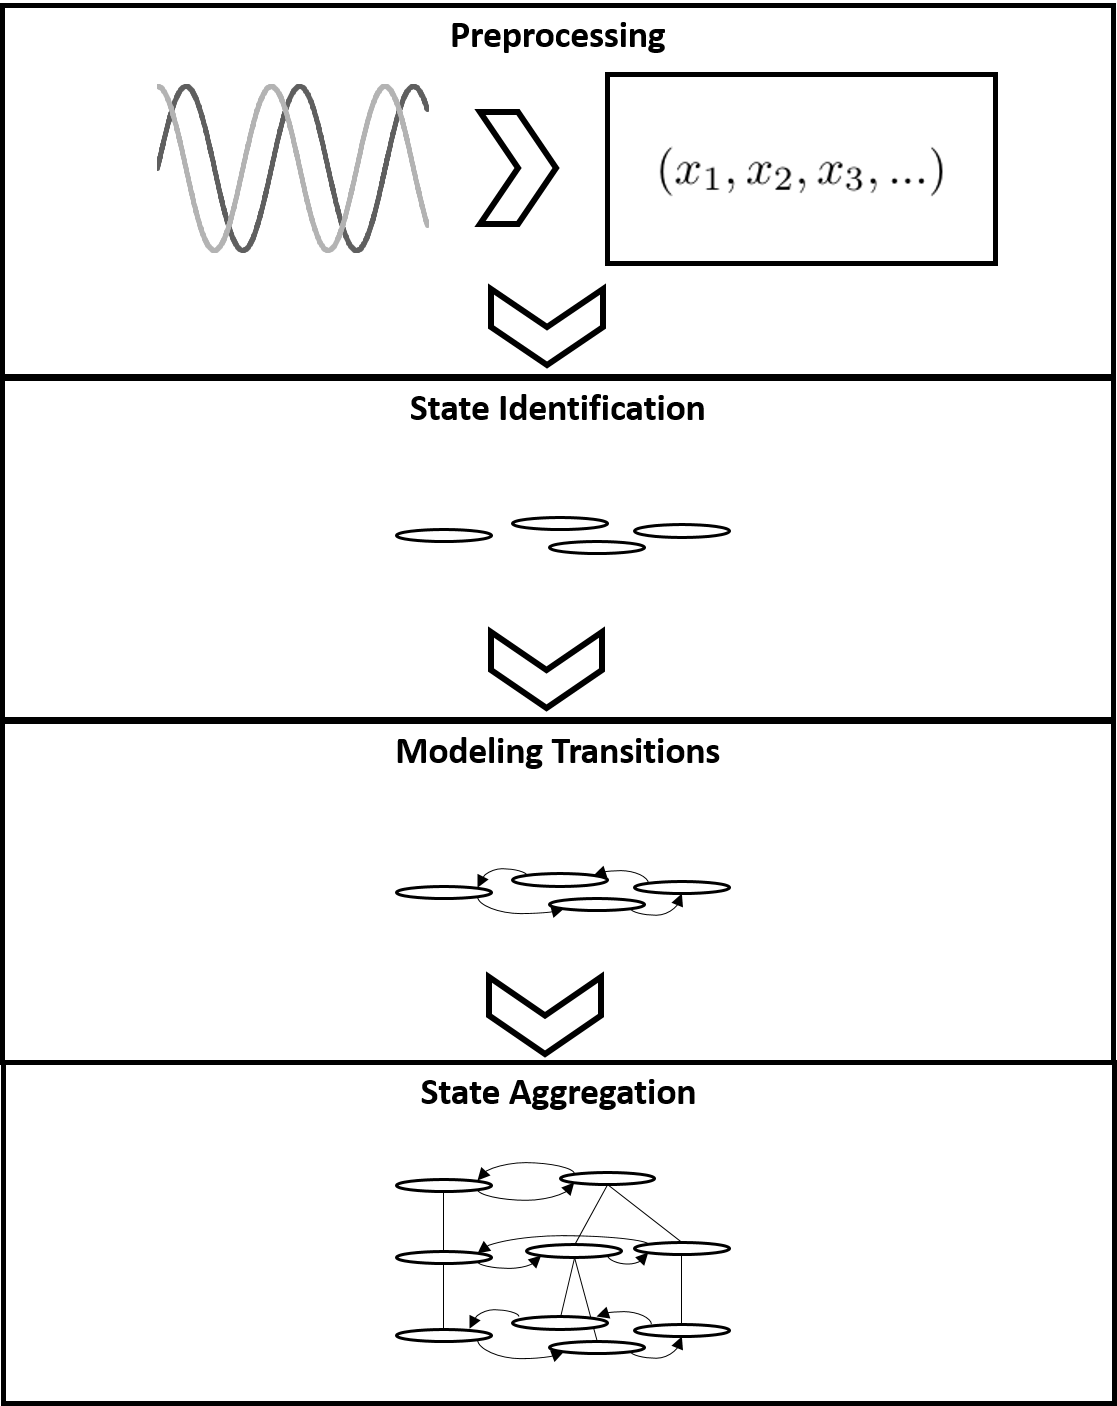
\includegraphics[width=300pt]{methodology}}
	\caption{The proposed multi-level methodology.}
	\label{fig:methodology}
\end{figure}
As shown in the figure our methodology encompasses four main steps. These include:
\begin{enumerate}
	\label{label:procedure-high-level}
	\item \label{label:procedure-preprocessing} aggregating and resampling the input
	streams, interpolating wherever needed, producing feature vectors,
	\item clustering the feature vectors to obtain lowest-level states and computing 
	statistics on each state,
	\item aggregating lowest-level states into a state hierarchy and computing the level
	on which each aggregated state lives and
	\item modeling state transitions with respect to control attributes and computing
	statistics on transitions.
\end{enumerate}
Each of these steps will be presented in the next subsections in detail.

\subsection{Merging and Processing Data Streams}

In recent years much attention of the research community has been focused on a
class of applications where the data are modeled best not as persistent relations,
but rather as transient data streams \cite{Babcock:2002:MID:543613.543615}. Data 
streams differ from conventional batch data in two main aspects: (1) their elements arrive online, sequentially
and the system has no control over their order and (2) data streams are potentially unbounded.

As such a data stream can be defined as a sequence of pairs $(t_i,x_i)_{i \ge 0}$
where $t_i$ is the timestamp of the $i$-th example and $x_i$ is its value.
In the first step our methodology consumes a batch of data streams and preprocesses 
them to obtain feature vectors which can be used to model the data in further steps.
The preprocessing is done by first merging the data streams to produce feature vectors with
a common time stamp and later resampling them using a domain-specific appropriate sampling rate.
After the resampling step, the methodology foresees the calculation of domain specific features
which the user would like to use when modeling the data. The last step can include the addition of
generic features like current derivative or some domain specific calculation like perhaps
the number of times an attribute was above a threshold in a domain specific time window.

\subsection{State Identification}

Once the data is represented as feature vectors it is ready to be modeled. Our next step includes identifying 
typical low-level system states from the feature vectors created in step 1. We do this by partitioning 
the feature vectors and associating each state with a partition. There are many partitioning algorithms 
available in the literature including algorithms that produce hierarchical partitions. In general however
the computational complexity of these algorithms is $O(n^2)$ which renders them unsuitable for big data
scenarios.
We therefore propose a flat partition using k-means resulting in a Voronoi diagram on the data space and
enabling us to construct states by assigning feature vectors to the partition with the nearest centroid
and constructing a hierarchical representation later in the process.
We then collect statistics in the states including
\begin{list}{-}{}
	\item Distribution of attributes - we store the distribution of all the attributes in a state as a
	histogram. The number of bins in a histogram is a configuration parameter and should be based on domain
	knowledge.
	\item Mean value and median of each attribute inside a state.
	\item Percentiles for each attribute.
\end{list}
These statistics can be used when the model is applied in real-time and provide a clustering-based anomaly detection
technique.

 and later aggregate it do obtain a hierarchical partition.

\begin{comment}
\subsection{State Aggregation}
\label{sec:state-aggregation}

To be able to represent the data streams in a qualitative manner

Once the data streams are merged we construct a state hierarchy. We do this 
by constructing a dendrogram of the previously constructed feature vectors.
A dendrogram is a nested sequence of partitions with associated numerical
level and is thus ideal for our multi-level representation. The literature
proposes many algorithms for constructing dendrograms. These generally fall
into two groups \cite{Maimon:2005:DMK:1088958}: 
\begin{enumerate}
	\item \textbf{Agglomerative} - each object initially represents a cluster of its own. Clusters are
	then iteratively merged, until the desired structure is obtained.
	\item \textbf{Divisive} - when the procedure starts, all object belong to the same cluster. Then
	clusters are recursively divided into sub-clusters until the desired structure is obtained.
\end{enumerate}

In general however, the time complexity of agglomerative clustering algorithms
is $\Omega(n^2)$ \cite{Sibson01011973}, which is impractical for large datasets.
Thus we compute an initial set of partitions using k-means and use them as
singletons of the dendrogram as well as the lowest level state space in our methodology.

\end{comment}
\begin{comment}


 We
first partition the feature vectors into a set of $k$ partitions. While partitioning is an
NP complete problem, there are several methods available which compute an approximation
efficiently. These include k-means, k-modes, CLARA, DP-means, etc. \cite{6558109,DBLP:journals/corr/abs-1111-0352}.

In our methodology we choose k-means for its simplicity [TODO].

The algorithm outputs a set of $k$ centroids $c_i$ where 

We note that when using our methodology, the number of partitions should be selected
based on domain knowledge or user experience. For instance in the example below
we chose $k = 12$, one for each month in a year.



 using clustering. 

 The advantages of cluster
partitions come from their geometric properties.
We do this by
first partitioning the feature vectors obtaining a set of $k$ partitions. The literature
proposes many partitioning algorithms.
 Clustering is an
unsupervised machine learning procedure, which organizes a collection of patterns,
usually represented
\end{comment}

\subsection{Data Stream Partitioning}

[TODO zamenjaj zgornji naslov s trenutnim]

\subsection{Modeling Transitions}

We model transitions using a Markovian model. The main characteristics of Markovian
models is that they retain no memory of where they have been in the past. This means
that only the current state can influence where the process will go next. In this 
work we are interested only in processes that can assume a finite set of states, 
called Markov chains \cite{norris1998markov}.
More formally, we are interested in Markov chains $(X_t)_{t \ge 0}$ which can assume
values in a finite state space $S$. We define $p_{ij}(t)$ to be the probability of
the process being in state $j$ at time $t$ when starting from state $i$ at time $0$.
We define a stochastic matrix $P(t)$, where $(P(t))_{ij} = p_{ij}(t)$. Thus each row
of $P(t)$ is a probability distribution over the state space. Such a chain can be 
represented by a transition rate matrix $Q$, where $Q$ satisfies the following system
of equations
\begin{equation}
	\label{eq:q-matrix}
	\frac{d}{dt}P(t) = P(t)Q, \qquad P(0) = I.
\end{equation}
and has the following properties:
\begin{enumerate}
	\item $-\infty < q_{ii} \le 0$
	\item $q_{ij} \ge 0$ for $j \neq i$
	\item $\sum_{j \in S}q_{ij} = 0$
\end{enumerate}
Each non-diagonal entry of $Q$, $q_{ij}$ thus represents the rate of going from state $i$
to state $j$ while the diagonal entries $-q_{ii}$ represent the rate of leaving state $i$.

We assume that $P(t)$ is recurrent for all $t$ and define $\pi_j = \lim_{t \rightarrow \infty} p_{ij}(t)$.
It can be shown that for recurrent chains $\pi_j$ is independent of the starting state and
vector $\pi = (\pi_1, \pi_2, ..., \pi_k)$ is called the stationary distribution
of $(X_t)_{t \ge 0}$ and represents the proportion of time the process spends in 
each state after funning for an infinite amount of time.

Using this representation, the stationary distribution $\pi$ can be computed as the
left eigenvector of $Q$ corresponding to eigenvalue $0$.

\subsubsection{Transition Rate Estimation}

We estimate the transition rates of $(X_t)_{t \ge 0}$ by first discretizing the
the continuous parameter space $t \in \left[0,\infty\right)$ into a discrete 
sequence $(0, h, 2h, ...)$ and estimating the transition probabilities
$\tilde{p}_{ij} = p_{ij}(h)$. Once $\tilde{p}_{ij}$ are estimated, the transition
rates can be calculated as 
\begin{equation}
	q_{ij} = \frac{h}{\tilde{p}_{ij}}.
\end{equation}
As proposed in section \ref{sec:introduction} we allow the users to simulate
the dynamics based on an alternate configurations of the predefined attributes
which we denote $A_S$.
Suppose the process is in state $i$ at time $0$ and define a random variable
$J_i = j \Leftrightarrow X_h = j$. Thus $J_i$ has a multinomial distribution
with parameters $(p_{i1}, p_{i2}, ..., p_{in})$ which can be modeled using
a generalized linear model (GLM) \cite{glm-introduction}. Because there is
no natural ordering in the response category, we use nominal logistic regression
to estimate $p_{ij}$ based on values $x_k \in A_S$. We select reference category
as $p_{ii}$ and model the relationship between $x_k$ and $p_{ij}$ as follows:
\begin{equation}
	\logit(p_{ij}) = \log\left(\frac{p_{ij}}{p_{ii}}\right) = \beta_{ij} x_k
\end{equation}
thus, for each state we get a set of $n-1$ equations which are used simultaneously
to estimate the parameters $\beta_{ij}$. Once these have been obtained, the linear
predictors can be calculated as:
\begin{equation}
	\tilde{p}_{ij}(x_k) = \frac{e^{\beta_{ij}x_k}}{1 + \sum_{l \neq i}e^{\beta_{il}x_k}}.
\end{equation}

\subsection{State Aggregation}

Once the process is modeled on the lowest level, we aggregate states
to obtain a hierarchy of such processes. We define state aggregation as the problem
of partitioning a Markov chain and adapt the algorithm proposed in \cite{5160607} to
work in a continuous time setting. Let a 
Markov chain on a state space $X$ be defined by a 
transition rate matrix $Q$. We define a surjective partition function $\phi: X \rightarrow Y$
and a corresponding transition rate matrix transformation function 
$\Phi: \mathbb{R}^{n \times n} \rightarrow \mathbb{R}^{m \times m}$ using the following formula:
\begin{equation}
	\Phi (Q) = (P'\Pi P)^{-1}P'\Pi QP
\end{equation}
where $\Pi = diag(\pi)$ and $P$ is a $\left|X\right| \times \left|Y\right|$ partition matrix
with elements
\begin{equation}
	\left(P\right)_{ij} = 
	\left\{
		\begin{array}{ll}
			1 & \mbox{if } \phi(i) = j \\
			0 & \mbox{otherwise}.
		\end{array}
	\right.
\end{equation}
Thus once knowing the partition function on a specific detail level, the associated Markov chain
can be computed efficiently. We note however that information is lost when aggregating the state
space of a Markov chain and the original chain can never be computed from only the aggregated one.

Now that we can represent a Markov chain knowing a partition function, we present an algorithm
for partitioning such chains using spectral graph theory. We first propose a bi-partitioning
algorithm which is used recursively to split the aggregated states.

\subsubsection{Bi-Partitioning Markov Chains}
\label{sec:bi-partition}

The spectral analysis of undirected graphs has been studied extensively in the literature and
many algorithms for bi-partitioning such graphs proposed. These papers use the Cheeger
inequality, one of the main tools for bounding the mixing times for random walks on undirected
graphs, on the graph Laplacian. The transition rate matrix of a Markov chain is exactly the negative Laplacian
of a directed weighted graph $Q = -L(G)$ \cite{Agaev2005157}.
The Laplacian is however not symmetric and in general does not have real eigenvalues.
Therefore we transform the Laplacian using the following formula:
\begin{equation}
	Q_s = \frac{1}{2}(\Pi Q + Q'\Pi)
\end{equation}
The transformation above has the effect of symmetrizing the transition rate matrix and furthermore
the matrix $\Pi^{-1}Q_s$ preserves the ergodic properties of the original Markov chain. To
obtain a bi-partition of the original Markov chain we then solve the following generalized eigenvalue
problem:
\begin{equation}
	Q_s v = \lambda_2 \Pi v
\end{equation}
The bi-partition function $\phi$ is then constructed using the following rule:
\begin{equation}
	\phi(i) = 
	\left\{
		\begin{array}{ll}
			1 & \mbox{if } v_i \ge 0 \\
			0 & \mbox{otherwise}
		\end{array}
	\right.
\end{equation}

\subsubsection{Partitioning Markov Chains}

Since the bi-partitioning problem can be solved using the second eigenvector of the transformed
Laplacian we can now present a recursive algorithm for the partitioning of continuous time Markov chains.
We first define the entropy rate function
\begin{equation}
	D(Q||\tilde{Q}) = \sum_{A \in \Ima \phi}\sum_{B \in \Ima \phi}\sum_{i \in \phi^{-1}(A)}\pi_i \sum_{j \in \phi^{-1}(B)} q_{ij} \log \frac{\sum_{j \in \phi^{-1}(B)} q_{ij}}{\tilde{q}_{AB}}
\end{equation}
[TODO entropy rate not yet developed]

There are a couple of options to calculate the distance between Markov chains:
\begin{list}{-}{}
	\item Wasserstein
	\item Total Variation
	\item Entropy rat
\end{list}

The algorithm starts with an initial partition containing all the states of the original Markov chain.
On the $n$-th iteration the algorithm assumes that $n$ partitions (aggregated states) are given. The objective then is
to select the best aggregated state to split, obtaining $n+1$ partitions. For $i=1,2, ..., n$ we denote $Q^{(i)}$ to
be the transition rate matrix of a Markov chain within the $i$-th partition. A bi-partition of $Q^{(i)}$
provides $n+1$ partitions, which we denote $Q_{n+1}^{(i)}$. The objective then is to select the best 
partition $Q^{(i)}$ to split. This is achieved by minimizing the following criteria:
\begin{equation}
	\argmin_{i \in \{1, 2, ..., n\}} D(Q||Q_{n+1}^{(i)})
\end{equation}


\newpage



\begin{comment}
 The methods proposed
in these papers use the sign structure of the second largest eigenvalue as an approximate
solution of the bi-partitioning problem. However all these papers assume a symmetric Laplacian.




While the spectral analysis of undirected graphs has been studied extensively, there
are few papers discussing the spectral properties of directed graphs.

It has been shown that an approximate solution to the min-cut problem



In general partitioning is an NP-complete problem, however in the pioneering
work of Wentzell and Freidin it is shown that an optimal aggregation is 
obtained through the sign structure of the second eigenvector.

In the work of Wentzell and Freidlin it is shown that an optimal aggregation
is obtained through the sign structure of the second eigenvector.

The partitioning of a continuous time Markov chain can
be viewed as an optimization problem where we minimize the total relative 
entropy between a Markov chain Q and an aggregated chain  where
the partition function $\pi : S \rightarrow S$ is defined by:



Recall from section \ref{sec:state-aggregation} that our methodology
partitions the data space using a dendrogram. A dendrogram is a nested sequence
of partitions with associated numerical levels. Thus it provides, on each level $l$,
a unique partition of the data space $P^l = (P_1, P_2, ... P_{k_l})$ where each partition
$P_i$ is the union of one or more partitions on level $0$. Since each state of the 
Markov chain corresponds to a single partition on level $0$, we aggregate
then to be able model the higher level process on level $l$. Suppose
the data space is partitioned into partitions $(P_1, P_2, ..., P_k)$ on level $0$.

We note that simply lumping lower level states is not sufficient since it may
result in a non-Markovian process [TODO ref]. Therefore we construct a new
Markov chain $(Y_t)_{t \ge 0}$ which should retain some the behavior of the original
chain $(X_t)_{t \ge 0}$. Let $(X_t)_{t \ge 0}$ be the Markov chain on level $0$ with state space $S = {1, 2, ..., n}$
and transition rate matrix $Q$. Now suppose we would like to aggregate two sets of 
states  $A = \{i_1, i_2, ..., i_k\} \subset S$ and $B = \{j_1, j_2, ..., j_h\} \subset S$
and would like to preserve the stationary distribution of the original process. Let
$\tilde{\pi}$ be the stationary distribution of $(Y_t)_{t \ge 0}$. Then $\tilde{\pi}$
should have the following properties:
\begin{enumerate}
	\item $\tilde{\pi}_A = \sum_{i \in A}\pi_i$, $\tilde{\pi}_B = \sum_{j \in B}\pi_j$
	\item $\tilde{\pi}_k = \pi_k$ for all $k \notin A \cup B$.
\end{enumerate}
We can compute the transition rate matrix of such a process using the following 
formula:
\begin{equation}
	q_{AB} = \frac{\sum_{i \in A}\pi_i\sum_{j \in B}q_{ij}}{\sum_{i \in A}\pi_i}.
\end{equation}

[TODO ta formula je dokazana v clanku ki ga imas + se DTMC partitioning, 
mogoce lahko partitioning razsiris na CTMC, vrzes ven trenutni dendrogram
in to opsises v clanku]

\end{comment}

\subsection{Visualization}

In the user interface, the model is presented on only one level of the hierarchy. States are presented
as circles while transitions are presented as arrows between states. The area of each state is proportional to
the mean time the process spends in the state which is extracted from the stationary distribution of the
Markov chain on the current detail level. The user can zoom into and out of
more detailed levels by using the zoom function. We offer several services that allow the users to identify
the meaning of states, which are presented in Section \ref{sec:ui}.

To visualize states, their planar coordinates are precomputed by the state identification component. This
is achieved by computing the initial or seed positions using principal component analysis (PCA) on the
state centroids. To avoid state overlap, we then refine state positions using a repulsive-simulation based
technique across all the detail levels simultaneously.

\begin{comment}

\section{Theory}

This section presents the theory behind the StreamStory systems. We begin with
a general discussion about data streams, then we give some insight into the 
theory behind clustering algorithms and stochastic processes.

\begin{comment}
High dimensional systems arise in a variety of applications. In many cases these are
stochastic by nature or can be well approximated by stochastic processes. Other systems
that model high dimensional data include systems that model the system as a Markovian 
state model [TODO ref] and milestoning [TODO ref]. There are also several other techniques
[TODO ref] [TODO razdelaj].

Data streams can be defined by a set of tuples $(t_i, x_i)$, where $t_i$ represents
the timestamp of the $i$-th observation $x_i$. They can be characterized by the following:
\begin{enumerate}
	\item the elements of the data stream arrive sequentially, and the developer
	has no control over their timing,
	\item each stream can provide elements at its own schedule: they do not need
	to have the same data rates or types
	\item a data stream is potentially unbounded in size.
\end{enumerate}
A data stream may contain sensor data, image data or maybe internet and web traffic.
High dimensional data streams arise in many applications. In many cases these
are stochastic in nature or can be approximated by a stochastic process \cite{2014arXiv1404.0667C}.

One of the major challenges when modeling such processes is the ability to reach
experimentally relevant timescales \cite{pande-beauchamp-bowman:2010:methods:markov-model-review}.

Markov state models build models with $N$ states and parametrize the model with the
rates between states. The challenges when building Markov state models include \cite{pande-beauchamp-bowman:2010:methods:markov-model-review}:
\begin{enumerate}
	\item defining the states of the model and
	\item using the state decomposition to build a transition matrix in an efficient
	manner.
\end{enumerate}

To define the models' states, we chose to partition the data streams.

\subsection{Gaussian Mixture Models and K-means}

A mixture model is a probabilistic model that represents the presents of subpopulations
in an observed population. A mixture model corresponds to a mixture distribution
that represents the distribution of observations in the overall population.
In a Gaussian mixture model, the data is assumed to arise from the following distribution:
\begin{equation}
	\label{eq:gaussian-mixture}
	p(x) = \sum_{i=1}^{k}\pi_i N(\mu_i, \Sigma_i)
\end{equation}
where $k$ is the number of components, $\pi$ is the mixing coefficient and $\mu_i$ and
$\Sigma_i$ are parameters of a Gaussian distribution. \textcolor{yellow}{[TODO]}
A related model is provided by the K-means objective function, which constructs a 
hard partitioning of the data set. Given a set of points $x_1, x_2, ..., x_n$, the 
K-means objective function attempts to find partitions $c_1, c_2, ..., c_k$ that
minimize the following objective function:

\newcommand{\norm}[1]{\left\lVert#1\right\rVert}

\begin{equation}
	\label{eq:k-means-obj}
	\min_{bounds} \sum_{j = 1}^{k}\sum_{x_i \in r(j)} \norm{x_i - \mu_j}_2^2
	where \mu_j = \frac{1}{|r(j)|}\sum_{x_i \in r(j)} x_i
\end{equation}

\subsection{What is left}

Once the model is build it can be used for quantitative simulations as well as
qualitative interpretation.

To define the models' states, we use 

% Head 1
\section{Implementation}

This section presents the detailed implementation of the StreamStory system, by 
presenting in details each step of our four step process. We begin the section
by first discussing the preprocessing step proposed in step \ref{label:procedure-preprocessing} 
of our four step process defined in section \ref{sec:introduction}.

% Head 2
\subsection{Data Stream Aggregation and Resampling}

In recent years much attention in the research community has been focused on a new
class of applications: applications in which the data is modeled best not as persistent
relations but rather as transient data stream \cite{Babcock:2002:MID:543613.543615}.

Data streams differ from conventional batch data in several ways:
\begin{list}{-}{}
	\item the data elements arrive online, sequentially and the system has no control
	over their order and
	\item data streams are potentially unbounded.
\end{list}

As such a data stream can be defined as a sequence of pairs $(t_i,x_i)_{i \ge 0}$, 
where $t_i$ represents the timestamp if the $i$-th measurement and $x_i$ represents 
its value. In our work we assume the streams follow the following model: 
$x_{i+1} = x_i + X$, where $X$ is a normally distributed random variable $X \sim N(\mu, \sigma)$.
\textcolor{red}{[TODO really???]}

To build a model in offline mode, StreamStory consumes batches of multiple such
data streams and merges them, to that all the stream are sampled at the same timestamps.
This results in a single joined data stream in the following form:

\begin{equation}
	\nonumber
	\left\{\left(t_1, x_1^{(1)}, x_1^{(2)}, ..., x_1^{(d)}\right), \left(t_1 + \Delta t, x_2^{(1)}, x_2^{(2)}, ..., x_2^{(d)}\right), ..., \left(t_0 + (k-1)\Delta t, x_k^{(1)}, x_k^{(2)}, ..., x_k^{(d)}\right)\right\}
\end{equation}

Since in general not all the input streams are equally sampled, missing values need
to be interpolated. For this purpose StreamStory supports two interpolation methods:
linear and previous point interpolation. The choice of the interpolation method
influences the online behavior of the system. Although in theory linear interpolation
produces better results \textcolor{red}{[TODO ref]}, linear interpolation cannot 
interpolate a value until it observes at least one value in the \textcolor{red}{[TODO future]}.
Which results in a certain lag (non-real-time behavior) of the system.

\subsection{State Identification}

Once the data streams are preprocessed, StreamStory identifies their typical lowest-level
states. This is achieved by clustering the joined data stream.

Clustering is an unsupervised machine learning procedure, which organizes a collection
of patterns, usually represented as a vectors of measurements or points in a 
multidimensional space, into clusters based on a chosen measure of similarity or distance 
\cite{Jain:1999:DCR:331499.331504}. There is no universally agreed upon definition of a 
cluster. Most researchers describe it by considering the internal homogeneity and 
external separation \cite{1427769}.

Intuitively patterns in the same cluster should be more similar to each other than to patterns
in other clusters. There are many clustering algorithms that solve different problems. These 
include partitioning, \textcolor{red}{[TODO]}.

We support two partitioning methods: K-Means and DPMeans. The first is a well studied method
which, given $k$ - the desired number of clusters, partitions the dataset into $k$ clusters by 
minimizing the distance between data points and the nearest centroid \cite{kmeans}. It works
by, initially selecting $k$ random centroids, then in each iteration it first assigns all the 
feature vectors to their nearest centroid constructing a Voronoi diagram regions are associated
with centroids $C = \left\{c_1, c_2, ..., c_k\right\}$. More formally a region of the diagram
is defined as $R(c_i) = \left\{x \in \mathbb{R}^d | d(c_i,x) \le d(c_j,x) \: \forall j\right\}$.
The method then recomputes each centroid $c_i$ as the mean value of all the data points that lie
in region $R(c_i)$:

\begin{equation}
	\label{eq:kmeans-centroids}
	\nonumber
	c_i = \frac{1}{\|R_i\|}\sum\limits_{p_j \in R(c_i)}p_j.
\end{equation}

The procedure terminates when the partitions are the same in two consecutive iterations.

The second method, DP-means, proposed by \cite{DBLP:journals/corr/abs-1111-0352} behaves
similarly to K-Means with the exception that a new cluster is formed whenever a feature
vector is further than $\lambda$ away from every existing centroid. Thus, the number of 
clusters on the output is not known in advance, but is controlled by $\lambda$.

When identifying states, we first remove timestamps from the joined data stream, resulting 
in feature vectors of the form 

\begin{equation}
	\nonumber
	x_i = \left(x_i^{(1)}, x_i^{(2)}, ..., x_i^{(d)}\right).
\end{equation}

These are then clustered using one of the above methods, resulting in a set
of $k$ partitions which are used as lowest level states. When StreamStory \textcolor{red}{[TODO sees]}
a new data point it will assign it to the state (partition) with the nearest centroid.
\begin{equation}
	\label{eq:low-level-assignment}
	\nonumber
	S(p_i) = \argmin_{p_j \in R(c_j)} d(p_i, c_j)
\end{equation}
Where $d$ represents the Euclidean distance.

\subsection{State Aggregation}

Once the lowest level states are computed, StreamStory aggregates them into a state hierarchy.
Before grouping states, we need to measure their relative distance to each other. Since StreamStory
was developed to work with dense dataset, we use the Euclidean distance. Many hierarchical
clustering techniques have been proposed in the literature. They can be characterized
as greedy in the algorithmic sense \cite{DBLP:journals/corr/abs-1105-0121}. Assuming that a pair
of states is merged or agglomerated at each step, the techniques construct a binary tree
commonly known as a dendrogram. This produces a set of states at each level - or each threshold 
value which produces a new partition. Hierarchical clustering methods generally fall into two
groups \cite{Maimon:2005:DMK:1088958}: 
\begin{list}{-}{}
	\item \textbf{Agglomerative} - each object initially represents a cluster of its own. Clusters are
	then iteratively merged, until the desired structure is obtained.
	\item \textbf{Divisive} - when the procedure starts, all object belong to the same cluster. Then
	clusters are recursively divided into sub-clusters until the desired structure is obtained.
\end{list}
These groups can be further subdivided according to the manner that the distance measure is
calculated:
\begin{list}{-}{}
	\item \textbf{Single-link} - methods that consider the distance between two clusters equal to the
	minimum distance of any member of one cluster to any member of the other.
	\item \textbf{Complete-link} - methods that consider the distance between two clusters equal to
	the maximum distance of any member of one cluster to any member of the other.
	\item \textbf{Complete-line} - methods that consider the distance between two clusters equal to
	the average distance of any member of one cluster to any member of the other.
\end{list}
StreamStory uses an agglomerative clustering technique and supports all three of the above
mentioned linkage strategies.

\subsection{Modeling Transitions}

% TODO theory and implementation razlicna
% teorija
% nato implementacija
% zvezni proces v evklidskem prostory
% how to do data mining
% nikoli ne recoveramo zveznega procesa (remark)

We model transitions using a Markovian model. The main characteristic of Markovian models
is that they retain no memory of where they have been in the past. This means that only the
current state can influence where the process will go next. In this work, we are interested
only in processes that can assume a finite set of states, called Markov chains \cite{norris1998markov}.

More formally, we are interested in Markov chains $(X_k)_{k \ge 0}$, which can assume 
values in a finite state space $S$. We define $p_{ij}(k) = P(X_k = j | X_0 = i)$ to be the probability
of the process being in state $j$ at time $k$ when starting from state $i$ at time $0$.
Because of the memoryless property $P(X_k = j | X_0 = i) = P(X_{k+m} = j | X_m = i) = p_{ij}(k)$.

We define a stochastic matrix $P(t)$, where $\left(P(t)\right)_{ij} = p_{ij}(t)$. Thus the
$i$-th row of $P(t)$ is a probability distribution over the state space at time $t$
when the process starts from state $i$. We assume that $P(t)$ is recurrent and define 
$\pi_j = \lim\limits_{t \rightarrow \infty} p_{ij}(t)$. Then $\pi = \left(\pi_1, \pi_2, ..., \pi_m\right)$
is the stationary distribution of $\left(X_t\right)_{t \ge 0}$ and represents the proportion
of time the process spends in each state after running for an infinite amount of time.

Let us now observe the elements if $P(t)$. Since each row of $P(t)$ is a probability
distribution it is clear that $p_{ij}(t) \ge 0$ and $\sum_{j \in S}p_{ij}(t) = 1$.
Furthermore $p_{ij}(t)$ must satisfy the memoryless property $P(X_{t+s} = j | X_s = i) = p_{ij}(t)$.

\subsubsection{State Aggregation}

When observing the process on multiple resolutions we need a way to aggregate states
in $S$. When aggregating states of the Markov chain, we choose a formula which preserves
the stationary distribution. Suppose $A$ and $B$ are non-intersecting subsets of $S$.
Then we can calculate the probability of the process going from set $A$ to set $B$ for any
$t$ as follows:
\begin{equation}
	\label{eq:markov-aggregation}
	p_{AB}(t) = \frac{\sum\pi_i\sum_{j \in A}p_{ij}(t)}{\sum_{i \in B}\pi_i}
\end{equation}



\begin{comment}


What makes these processes useful is that not only do they model many phenomena of interest,
but also the lack of memory property makes it possible to predict how a Markov chain may
behave, and to compute probabilities and expected values which quantify that behavior
\cite{norris1998markov}.
We define a Markov chain as a memoryless stochastic process $\left(X_k\right)_{k \ge 0}$
that can assume a finite set of states $i \in I$, where $I$ is called the state space.


Discrete time Markov chains move in discrete time steps. They are defined using a 
stochastic matrix $P$ where $(P)_{ij} = p_{ij}$ is the probability of jumping from state
$i \in I$ to state $j \in I$ in a single time step. More formally we say that a stochastic
process $\left(X_n\right)_{n \ge 0}$ is a discrete time Markov chain with initial distribution
$\lambda$ if
\begin{enumerate}
	\item $X_0$ has distribution $\lambda$ and
	\item $P(X_{n+1} = i_{n+1} | X_0 = i_0, X_1 = i_1, ..., X_n = i_n) = p_{i_ni_{n+1}}$
\end{enumerate}
Once of the interesting properties of Markov chains are their stationary distributions. A 
stationary distribution describes the proportion of time the process spends in each state.
In our visualization it represents the size of states. The stationary distribution can be
computed as the left eigenvector of $P$ with the corresponding eigenvalue 1.

When drawing the hierarchy we need some way of aggregating states in the Markov chain. 
Suppose we have two non-intersecting sets of states $A = \left\{j_1, j_2, ..., j_k\right\}$ and
$B = \left\{i_1, i_2, ..., i_h\right\}$. Then we use the following formula to compute
the transition probability from set $A$ to set $B$:
\begin{equation}
	\label{eq:dt-aggregation}
	\begin{split}
		p_{AB} = 
		P(X_{n+1} \in A | X_n \in B) = 
		\sum\limits_{j \in A}P(X_{n+1} = j | X_n \in B) = \\
		\sum_{j \in A}\frac{P(X_{n+1} = j)P(X_n \in B | X_{n+1} = j)}{P(X_n \in B)} = 
		\frac{\sum_{j \in A} \pi_j \sum_{i \in B}\frac{p_{ij}\pi_i}{\pi_j}}{\sum_{j \in B} \pi_i} = \\
		\frac{\sum_{i \in B}\pi_i\sum_{j \in A}p_{ij}}{\sum_{j \in B} \pi_i}
	\end{split}
\end{equation}

A natural way of interpolating discrete time steps $\left(p^n\right)_{n \in \mathbb{N}}$ is by the
exponential function $\left(e^{tq}\right)_{t \in \mathbb{R}^{+}}$. Consider a finite state set $I$ and a stochastic
matrix $P$. For any matrix $Q = (q_ij)_{i,j \in I}$, the series
\begin{equation}
	\sum_{k=0}^{\infty}\frac{Q^k}{k!}
\end{equation}
converges componentwise to $e^Q$. Now suppose that we can find a matrix $Q$ such that $e^Q = P$. Then
$e^{nQ} = (e^Q)^n = P^n$, so $\left(e^{tq}\right)_{t \in \mathbb{R}^{+}}$ fills the gaps in the 
discrete sequence.

If we now set $P(t) = e^{tQ}$, then $P(t)$ has the following properties:
\begin{enumerate}
	\item $P(s+t) = P(s)P(t)$
	\item $P(t)$ is the unique solution to equations $P'(t) = P(t)Q$ and $P'(t) = QP(t)$ with
	initial condition $P(0) = I$.
\end{enumerate}

\subsection{Visualization}

\end{comment}

\section{Visualization and User Interaction}
\label{sec:ui}

When interacting with the StreamStory system, the user is presented with a two panel user interface
shown in Figure \ref{fig:ui-initial}.
 
\begin{figure}[h!]
	\centering
	\makebox[\textwidth]{\includegraphics[width=\textwidth]{ui-initial}}
	\caption{User interface of the StreamStory system.}
	\label{fig:ui-initial}
\end{figure}

The visualization panel on the left visualizes the hierarchical Markovian model. States are 
represented by circles, while transitions are represented by arrows. The size of a state
is proportional to the fraction of time the monitored process spends in the state. When 
StreamStory is used in online mode, the current state is colored green, the most likely
future states blue and the previous state has a red border.

The thickness of an arrow is proportional to the probability of the corresponding transition,
and the most likely transitions have a darker color.

When first opening user interface the user is presented with a top-level chain with only two 
states. They can then use the scroll function to zoom into the hierarchy and the states are expanded
automatically.

Users can view a state by using the click function. By doing this, the state becomes selected and
the user is presented with several services that assist them in identifying the meaning of the state.
These will be presented shortly in the following subsections.

\subsection{State Details and Attribute Highlighting}

\begin{list}{-}{}
	\item Histograms
	\item Means values, median
	\item Percentiles
	\item Suggesting attributes that are unique to the state - logistic regression weight extraction - classifying instances of the selected state against instances of other states
\end{list}

\subsection{Decision Trees}
\label{sec:ui-decision-trees}

The next state assist service are decision trees. Decision trees are classification models
often used in domains such as medicine for their explanatory power. When a decision tree
is induced, a split attribute and cut value are chosen recursively by a design time
criteria. The user can then interpret the tree by traversing the path from the root
to one of the leafs.

We use decision trees as a tool that assists users identify the meaning of a state. To do this,
we induce a single decision tree per state, by classifying instances of the selected state
against the instances of all the other states thus obtaining a qualitative description of the
state and displaying it to the end user upon request. We show an example of a decision tree
describing a middle detail level state which we identified as summer in the England temperature
dataset in Figure \ref{fig:ui-decision-tree}.

\begin{figure}[h!]
	\centering
	\makebox[\textwidth]{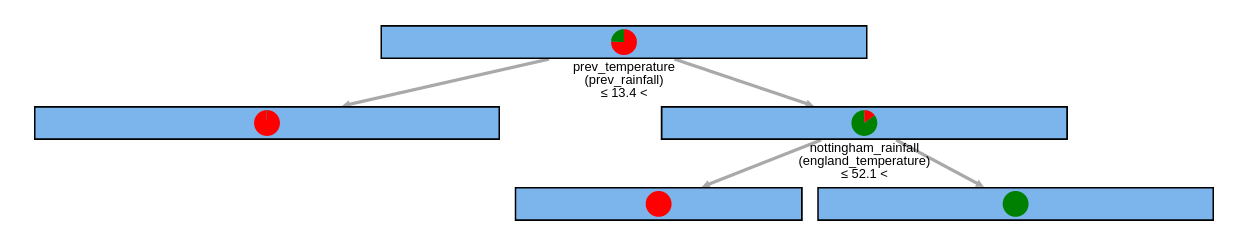
\includegraphics[width=\textwidth]{decision-tree}}
	\caption{An example tree describing a state in our user interface.}
	\label{fig:ui-decision-tree}
\end{figure}

Let us now observe what happens when inducing a decision tree and two attributes, for example $A$ 
and $B$ take exactly the same values when splitting a node. One of the two attributes, for 
example $A$ will be selected
as the split attribute. All the instances with the value of $A$ (and therefore also $B$) less
than the cut value will be passed to the left child, while all the instances with value of $A$ (also $B$) greater than the cut value will be passed to the right child. If this happens multiple
times when inducing the tree, the descriptive power of attribute $B$ can be totally neutralized
even though both attributes have the same meaning.

We avoid this problem by calculating the correlation between each of the attributes with the
split attribute and, if the correlation is high enough, display it as an alternate split in the 
visualization.

\subsection{Rule Extraction}

The next step is to display human readable rules that describe states. We do this by extracting
rules out of the decision trees described in Section \ref{sec:ui-decision-trees} using a recursive
algorithm. An example of a rule describing the "Summer" state presented above is shown in Figure 
\ref{fig:ui-rules}.

\begin{figure}[h!]
	\centering
	\makebox[\textwidth]{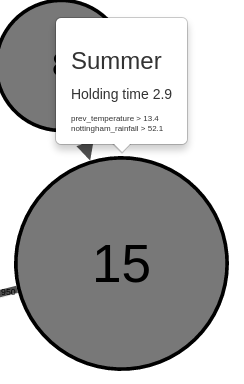
\includegraphics[width=200pt]{rules}}
	\caption{A rule extracted from the above presented decision tree describing the summer
	middle level state of the England temperature dataset.}
	\label{fig:ui-rules}
\end{figure}

The rules are extracted as a union of intersections using a recursive algorithm. The algorithm
works by creating initial intersection at the leafs which have a majority of positive instances.
It then traverses the tree upwards adding conditions to the intersection as it passes a node with 
only one intersection and creating a union of intersections when traversing a node with 
intersection on both its children.

\section{Experimantal Results}
\label{sec:experiment}

\section{Conclusion and Future Work}
\label{sec:conclusion}


\begin{comment}
By clicking on a state, the state becomes selected and its details are shown in the "Details"
panel on the right side of figure \ref{fig:ui-initial}. The details panel allows the user
to name the state which, we believe, increases the models interpretability. It also
shows the distribution of all the parameters inside the state as well as the mean value
of each parameter in the state. The mean value is highlighted red or green depending on
how specific the value is for that state. If the value is gray it means that the
value of the attribute is normal compared to the value of the same attribute in other 
states. However, if the value is green or red, it indicates the value is the value is
specific for this state compared to other states.

This is achieved by classifying the instances of the selected state against instances off
all the other states on the same level using a logistic regression model [TODO ref] and 
extracting weights. Values highlighted green indicate a positive weight, while values
highlighted red indicate a negative weight.
\end{comment}



















\begin{comment}
\newpage

We propose a suboptimal distribution to be used by each node, which is
easy to compute and does not depend on the number of competing
nodes. A natural candidate is an increasing geometric sequence, in
which
% Numbered Equation
\begin{equation}
\label{eqn:01}
P(t)=\frac{b^{\frac{t+1}{T+1}}-b^{\frac{t}{T+1}}}{b-1},
\end{equation}
where $t=0,{\ldots}\,,T$, and $b$ is a number greater than $1$.

In our algorithm, we use the suboptimal approach for simplicity and
generality. We need to make the distribution of the selected back-off
time slice at each node conform to what is shown in Equation
(\ref{eqn:01}). It is implemented as follows: First, a random
variable $\alpha$ with a uniform distribution within the interval
$(0, 1)$ is generated on each node, then time slice $i$ is selected
according to the following equation:
% Unnumbered Equation
\[
i=\lfloor(T+1)\log_b[\alpha(b-1)+1]\rfloor.
\]
It can be easily proven that the distribution of $i$ conforms to Equation
(\ref{eqn:01}).

So protocols [Bahl 2002,Culler 2001,Zhou 2006,Adya 2001,Culler 2001;
Tzamaloukas-01; Akyildiz-01] that use RTS/CTS
controls\footnote{RTS/CTS controls are required to be implemented by
802.11-compliant devices. They can be used as an optional mechanism
to avoid Hidden Terminal Problems in the 802.11 standard and
protocols based on those similar to [Akyildiz 2001] and
[Adya 2001].} for frequency negotiation and reservation are not
suitable for WSN applications, even though they exhibit good
performance in general wireless ad hoc
networks.

% Head 3
\subsubsection{Exclusive Frequency Assignment}

In exclusive frequency assignment, nodes first exchange their IDs
among two communication hops so that each node knows its two-hop
neighbors' IDs. In the second broadcast, each node beacons all
neighbors' IDs it has collected during the first broadcast period.

% Head 4
\paragraph{Eavesdropping}

Even though the even selection scheme leads to even sharing of
available frequencies among any two-hop neighborhood, it involves a
number of two-hop broadcasts. To reduce the communication cost, we
propose a lightweight eavesdropping scheme.

\subsection{Basic Notations}

As Algorithm~\ref{alg:one} states, for each frequency
number, each node calculates a random number (${\textit{Rnd}}_{\alpha}$) for
itself and a random number (${\textit{Rnd}}_{\beta}$) for each of its two-hop
neighbors with the same pseudorandom number generator.
% Algorithm
\begin{algorithm}[t]
\SetAlgoNoLine
\KwIn{Node $\alpha$'s ID ($ID_{\alpha}$), and node $\alpha$'s
neighbors' IDs within two communication hops.}
\KwOut{The frequency number ($FreNum_{\alpha}$) node $\alpha$ gets assigned.}
$index$ = 0; $FreNum_{\alpha}$ = -1\;
\Repeat{$FreNum_{\alpha} > -1$}{
        $Rnd_{\alpha}$ = Random($ID_{\alpha}$, $index$)\;
        $Found$ = $TRUE$\;
        \For{each node $\beta$ in $\alpha$'s two communication hops
    }{
      $Rnd_{\beta}$ = Random($ID_{\beta}$, $index$)\;
      \If{($Rnd_{\alpha} < Rnd_{\beta}$) \text{or} ($Rnd_{\alpha}$ ==
          $Rnd_{\beta}$ \text{and} $ID_{\alpha} < ID_{\beta}$)\;
      }{
        $Found$ = $FALSE$; break\;
      }
        }
     \eIf{$Found$}{
           $FreNum_{\alpha}$ = $index$\;
         }{
           $index$ ++\;
     }
      }
\caption{Frequency Number Computation}
\label{alg:one}
\end{algorithm}

Bus masters are divided into two disjoint sets, $\mathcal{M}_{RT}$
and $\mathcal{M}_{NRT}$.
% description
\begin{description}
\item[RT Masters]
$\mathcal{M}_{RT}=\{ \vec{m}_{1},\dots,\vec{m}_{n}\}$ denotes the
$n$ RT masters issuing real-time constrained requests. To model the
current request issued by an $\vec{m}_{i}$ in $\mathcal{M}_{RT}$,
three parameters---the recurrence time $(r_i)$, the service cycle
$(c_i)$, and the relative deadline $(d_i)$---are used, with their
relationships.
\item[NRT Masters]
$\mathcal{M}_{NRT}=\{ \vec{m}_{n+1},\dots,\vec{m}_{n+m}\}$ is a set
of $m$ masters issuing nonreal-time constrained requests. In our
model, each $\vec{m}_{j}$ in $\mathcal{M}_{NRT}$ needs only one
parameter, the service cycle, to model the current request it
issues.
\end{description}

Here, a question may arise, since each node has a global ID. Why
don't we just map nodes' IDs within two hops into a group of
frequency numbers and assign those numbers to all nodes within two
hops?

\section{Simulator}
\label{sec:sim}

If the model checker requests successors of a state which are not
created yet, the state space uses the simulator to create the
successors on-the-fly. To create successor states the simulator
conducts the following steps.
% enumerate
\begin{enumerate}
\item Load state into microcontroller model.
\item Determine assignments needed for resolving nondeterminism.
\item For each assignment.
      \begin{enumerate}
      \item either call interrupt handler or simulate effect of next instruction, or
      \item evaluate truth values of atomic propositions.
      \end{enumerate}
\item Return resulting states.
\end{enumerate}
Figure~\ref{fig:one} shows a typical microcontroller C program that
controls an automotive power window lift. The program is one of the
programs used in the case study described in Section~\ref{sec:sim}.
At first sight, the programs looks like an ANSI~C program. It
contains function calls, assignments, if clauses, and while loops.
% Figure
\begin{figure}
\centerline{
\includegraphics{acmsmall-mouse}}
\caption{Code before preprocessing.}
\label{fig:one}
\end{figure}

\subsection{Problem Formulation}

The objective of variable coalescence-based offset assignment is to find
both the coalescence scheme and the MWPC on the coalesced graph. We start
with a few definitions and lemmas for variable coalescence.

% Enunciations
\begin{definition}[Coalesced Node (C-Node)]A C-node is a set of
live ranges (webs) in the AG or IG that are coalesced. Nodes within the same
C-node cannot interfere with each other on the IG. Before any coalescing is
done, each live range is a C-node by itself.
\end{definition}

\begin{definition}[C-AG (Coalesced Access Graph)]The C-AG is the access
graph after node coalescence, which is composed of all C-nodes and C-edges.
\end{definition}

\begin{lemma}
The C-MWPC problem is NP-complete.
\end{lemma}
\begin{proof} C-MWPC can be easily reduced to the MWPC problem assuming a
coalescence graph without any edge or a fully connected interference graph.
Therefore, each C-node is an uncoalesced live range after value separation
and C-PC is equivalent to PC. A fully connected interference graph is made
possible when all live ranges interfere with each other. Thus, the C-MWPC
problem is NP-complete.
\end{proof}

\begin{lemma}[Lemma Subhead]The solution to the C-MWPC problem is no
worse than the solution to the MWPC.
\end{lemma}
\begin{proof}
Simply, any solution to the MWPC is also a solution to the
C-MWPC. But some solutions to C-MWPC may not apply to the MWPC (if any
coalescing were made).
\end{proof}

\section{Performance Evaluation}

During all the experiments, the Geographic Forwarding (GF)
[Akyildiz 2001] routing protocol is used. GF exploits geographic
information of nodes and conducts local data-forwarding to achieve
end-to-end routing. Our simulation is
configured according to the settings in
Table~\ref{tab:one}. Each run lasts for 2 minutes and
repeated 100 times. For each data value we present in the results,
we also give its 90\% confidence interval.
% Table
\begin{table}%
\tbl{Simulation Configuration\label{tab:one}}{%
\begin{tabular}{|l|l|}
\hline
TERRAIN{$^a$}   & (200m$\times$200m) Square\\\hline
Node Number     & 289\\\hline
Node Placement  & Uniform\\\hline
Application     & Many-to-Many/Gossip CBR Streams\\\hline
Payload Size    & 32 bytes\\\hline
Routing Layer   & GF\\\hline
MAC Layer       & CSMA/MMSN\\\hline
Radio Layer     & RADIO-ACCNOISE\\\hline
Radio Bandwidth & 250Kbps\\\hline
Radio Range     & 20m--45m\\\hline
\end{tabular}}
\begin{tabnote}%
\Note{Source:}{This is a table
sourcenote. This is a table sourcenote. This is a table
sourcenote.}
\vskip2pt
\Note{Note:}{This is a table footnote.}
\tabnoteentry{$^a$}{This is a table footnote. This is a
table footnote. This is a table footnote.}
\end{tabnote}%
\end{table}%

\section{Conclusions}

In this article, we develop the first multifrequency MAC protocol for
WSN applications in which each device adopts a
single radio transceiver. The different MAC design requirements for
WSNs and general wireless ad-hoc networks are
compared, and a complete WSN multifrequency MAC design (MMSN) is
put forth. During the MMSN design, we analyze and evaluate different
choices for frequency assignments and also discuss the nonuniform
back-off algorithms for the slotted media access design.

% Start of "Sample References" section



\section{Typical references in new ACM Reference Format}
A paginated journal article \cite{Abril07}, an enumerated
journal article \cite{Cohen07}, a reference to an entire issue \cite{JCohen96},
a monograph (whole book) \cite{Kosiur01}, a monograph/whole book in a series (see 2a in spec. document)
\cite{Harel79}, a divisible-book such as an anthology or compilation \cite{Editor00}
followed by the same example, however we only output the series if the volume number is given
\cite{Editor00a} (so Editor00a's series should NOT be present since it has no vol. no.),
a chapter in a divisible book \cite{Spector90}, a chapter in a divisible book
in a series \cite{Douglass98}, a multi-volume work as book \cite{Knuth97},
an article in a proceedings (of a conference, symposium, workshop for example)
(paginated proceedings article) \cite{Andler79}, a proceedings article
with all possible elements \cite{Smith10}, an example of an enumerated
proceedings article \cite{VanGundy07},
an informally published work \cite{Harel78}, a doctoral dissertation \cite{Clarkson85},
a master's thesis: \cite{anisi03}, an online document / world wide web resource \cite{Thornburg01}, \cite{Ablamowicz07},
\cite{Poker06}, a video game (Case 1) \cite{Obama08} and (Case 2) \cite{Novak03}
and \cite{Lee05} and (Case 3) a patent \cite{JoeScientist001},
work accepted for publication \cite{rous08}, 'YYYYb'-test for prolific author
\cite{SaeediMEJ10} and \cite{SaeediJETC10}. Other cites might contain
'duplicate' DOI and URLs (some SIAM articles) \cite{Kirschmer:2010:AEI:1958016.1958018}.
Boris / Barbara Beeton: multi-volume works as books
\cite{MR781536} and \cite{MR781537}.

\end{comment}

% Appendix
\appendix
\section*{APPENDIX}

\setcounter{section}{1}
\begin{comment}
In this appendix, we measure
the channel switching time of Micaz [CROSSBOW] sensor devices.
In our experiments, one mote alternatingly switches between Channels
11 and 12. Every time after the node switches to a channel, it sends
out a packet immediately and then changes to a new channel as soon
as the transmission is finished. We measure the
number of packets the test mote can send in 10 seconds, denoted as
$N_{1}$. In contrast, we also measure the same value of the test
mote without switching channels, denoted as $N_{2}$. We calculate
the channel-switching time $s$ as
\begin{eqnarray}%
s=\frac{10}{N_{1}}-\frac{10}{N_{2}}. \nonumber
\end{eqnarray}%
By repeating the experiments 100 times, we get the average
channel-switching time of Micaz motes: 24.3$\mu$s.
\end{comment}

\appendixhead{ZHOU}

% Acknowledgments
\begin{acks}
[TODO ackgnowledgements]
\begin{comment}
The authors would like to thank Dr. Maura Turolla of Telecom
Italia for providing specifications about the application scenario.
\end{comment}
\end{acks}

% Bibliography
\bibliographystyle{ACM-Reference-Format-Journals}
\bibliography{acmsmall-sample-bibfile}
                             % Sample .bib file with references that match those in
                             % the 'Specifications Document (V1.5)' as well containing
                             % 'legacy' bibs and bibs with 'alternate codings'.
                             % Gerry Murray - March 2012

% History dates
\received{February 2007}{March 2009}{June 2009}

% Electronic Appendix
\elecappendix

\medskip

\section{Distance Measure Between two Markov Chains}

We define a Markov chain $Q$ on a state space $X$, $\left|X\right| = n$, and a surjective partition function $\phi: X \rightarrow Y$, $\left|Y\right| = m$ with a corresponding partition matrix $P$. The transformed chain is then:

\begin{equation}
	\tilde{Q} = \left(P'\Pi P\right)^{-1}P'\Pi Q P
\end{equation}

We then have several options to measure the distance between $Q$ and $\tilde{Q}$.

\begin{equation}
	D_1(Q, \tilde{Q}) = \int\limits_{t = 0}^{\infty}\sum_{i=1}^{n}\sum_{j=1}^{n}\left|p_{i\phi(j)}(t) - \tilde{p}_{\phi(i)\phi(j)}(t)\right|dt
\end{equation}

\begin{equation}
	D_2(Q, \tilde{Q}) = \int\limits_{t = 0}^{\infty}\sum_{i=1}^{n}\sum_{j=1}^{n}\left(p_{i\phi(j)}(t) - \tilde{p}_{\phi(i)\phi(j)}(t)\right)^2 dt
\end{equation}

\begin{equation}
	D_3(Q, \tilde{Q}) = \int\limits_{t = 0}^{\infty}\sum_{i=1}^{n}\sum_{j=1}^{n}p_{ij}(t)\log{ \frac{p_{ij}(t)}{\tilde{p_{ij}}(t)}} dt
\end{equation}

\begin{equation}
	I(Q, \tilde{Q}) = \sum_{i=1}^{n}\sum_{j=1}^{n}p_{ij}(t)\log{ \frac{p_{ij}(t)}{\tilde{p_{ij}}(t)}} dt
\end{equation}

Where $p_{ij}(t) = \left(P(t)\right)_{ij} = \left(e^{Qt}\right)_{ij} = p_i'e^{Qt}p_j$ where $p_i$ is a vector with zeros everywhere except on the $i$-th position.
$Q$ can be decomposed using the eigen decomposition
\begin{equation}
	Q = V\Lambda V^{-1} = V\Lambda U
\end{equation}
with all eigenvalues $\lambda_i \le 0$ and exactly one eigenvalue $\lambda_z = 0$. The columns of $V$ are the right eigenvectors of Q.

Now let $v_i$ be the $i$-th row of $V$ and $u_j$ be the $j$-th column of $U$. We define 
$\psi(i) = \phi^{-1} \circ \phi(i)$ and:
\begin{eqnarray}
	v_{\phi(i)} &=& \frac{\sum_{k \in \psi(i)} \pi_k v_k}{\sum_{k \in \psi(i)} \pi_k} \\
	u_{\phi(i)} &=& \sum_{k \in \psi(i)} u_k
\end{eqnarray}
then $p_{ij}(t) = \left(e^{Qt}\right)_{ij} = p_i'e^{Qt}p_j$ can be written as:
\begin{eqnarray}
	p_{ij}(t) 
	&=& v_i e^{\Lambda t} u_j	\\ \nonumber 
	&=& \sum_{k \in X} v_{ik}e^{\lambda_k t} u_{kj}
\end{eqnarray}
$p_{i\phi(j)}(t)$ can be written as:
\begin{eqnarray}
	p_{i\phi(j)}(t) 
	&=& v_i e^{\Lambda t} u_{\phi(j)}	\\ \nonumber 
	&=& \sum_{k \in X} v_{ik}e^{\lambda_k t} u_{k \phi(j)} \\ \nonumber 
	&=& \sum_{k \in X}\sum_{l \in \psi(j)}v_{ik}e^{\lambda_k t} u_{kl} \\ \nonumber
	&=& \sum_{l \in \psi(j)}\sum_{k \in X} v_{ik}e^{\lambda_k t} u_{kl}
\end{eqnarray}
$p_{\phi(i)\phi(j)}(t)$ can be written as:
\begin{eqnarray}
	p_{\phi(i)\phi(j)}(t) &=& v_{\phi(i)} e^{\Lambda t} u_{\phi(j)} \\ \nonumber 
	&=& \sum_{k \in X} v_{\phi(i)k}e^{\lambda_k t} u_{k \phi(j)} \\ \nonumber
	&=& \frac{1}{\pi_{\psi(i)}}\sum_{k \in X}\sum_{h \in \psi(i)}\sum_{l \in \psi(j)}\pi_h v_{hk}e^{\lambda_k t}u_{kl} \\ \nonumber
	&=& \frac{1}{\pi_{\psi(i)}} \sum_{h \in \psi(i)}\pi_h\sum_{l \in \psi(j)}\sum_{k \in X} v_{hk}e^{\lambda_k t}u_{kl}
\end{eqnarray}
where $\pi_{\psi(i)} = \sum_{k \in \psi(i)}\pi_k$.

\subsection{Solving $I$}

We look at the equation for small $h$ for comparing the two chains in state space $Y$:

\begin{eqnarray}
	\label{eq:rel-entropy-orig}
	I(P(h), \tilde{P}(h)) &=& \sum_{\psi(i)}\sum_{\psi(j)}\pi_{\psi(i)}p_{\psi(i)\psi(j)}(h)\log\frac{p_{\psi(i)\psi(j)}(h)}{\tilde{p}_{\psi(i)\psi(j)}(h)}
\end{eqnarray}

We will modify this equation so that the original chain starts from a specific state $i$. The probability of starting from
$i$ if we know we are in $\psi(i)$ is $\frac{\pi_i}{\pi_{\psi(i)}}$. We modify equation \ref{eq:rel-entropy-orig}:

\begin{eqnarray}
	\label{eq:rel-entropy-mod}
	I(P(h), \tilde{P}(h))
		&=& \sum_{\psi(i)}\sum_{\psi(j)}\pi_{\psi(i)}\sum_{i \in \psi(i)}\frac{\pi_i}{\pi_{\psi(i)}}p_{i\psi(j)}(h)\log\frac{p_{i\psi(j)}(h)}{\tilde{p}_{\psi(i)\psi(j)}(h)} \\ \nonumber
		&=& \sum_{i}\sum_{\psi(j)}\pi_{i}p_{i\psi(j)}(h)\log\frac{p_{i\psi(j)}(h)}{\tilde{p}_{\psi(i)\psi(j)}(h)}
\end{eqnarray}

We know that $p_{i\psi(j)}(h) = \sum_{j \in \psi(j)}p_{ij}(h)$:

\begin{eqnarray}
	I(P(h), \tilde{P}(h))
		&=& \sum_{i}\sum_{\psi(j)}\pi_{i}\sum_{j \in \psi(j)}p_{ij}(h)\log\frac{\sum_{j \in \psi(j)}p_{ij}(h)}{\tilde{p}_{\psi(i)\psi(j)}(h)}
\end{eqnarray}

Now lets calculate this in terms of intensities $q_{ij}$. For small $h$ we can approximate $p_{ij}(h) \approx \delta_{ij} + q_{ij}h$, where 
$\delta$ is the Dirac function:

\begin{eqnarray}
	I(P(h), \tilde{P}(h))
		&\approx& \sum_{i}\sum_{\psi(j)}\pi_{i}\sum_{j \in \psi(j)}(\delta_{ij} + q_{ij}h)\log\frac{\sum_{j \in \psi(j)}(\delta_{ij} + q_{ij}h)}{\delta_{\psi(i)\psi(j)} + \tilde{q}_{ij}h}	\\	\nonumber	
		&=& \sum_{i}\sum_{\psi(j)} S_{i\psi(j)}
\end{eqnarray}

We now have 3 cases.

\subsubsection{Case 1: $i \neq j$, $i \not\in \psi(j)$}

In this case $\delta_{ij} = 0$ and $\delta_{\psi(i)\psi(j)} = 0$ and we get:

\begin{eqnarray}
	S_{i\psi(j)}
		&\approx& \pi_{i}\sum_{j \in \psi(j)}q_{ij}h\log\frac{\sum_{j \in \psi(j)}q_{ij}h}{\tilde{q_{ij}}h}	\\ \nonumber
		&=& \pi_{i}\sum_{j \in \psi(j)}q_{ij}h\log\frac{\sum_{j \in \psi(j)}q_{ij}}{\tilde{q}_{ij}}
\end{eqnarray}

Taking the derivative we get:
\begin{eqnarray}
	\frac{d}{dh}S_{i\psi(j)}
		&\approx& \pi_{i}\sum_{j \in \psi(j)}q_{ij}\log\frac{\sum_{j \in \psi(j)}q_{ij}}{\tilde{q}_{ij}}
\end{eqnarray}

Sending $h \downarrow 0$ we get the solution:
\begin{eqnarray}
	\lim_{h \downarrow 0}\frac{d}{dh}S_{i\psi(j)}
		&\approx& \pi_{i}\sum_{j \in \psi(j)}q_{ij}\log\frac{\sum_{j \in \psi(j)}q_{ij}}{\tilde{q}_{ij}}
\end{eqnarray}


\subsubsection{Case 2: $i \neq j$, $i \in \psi(j)$}
\label{sec:case2}

In this case $\sum_{j \in \psi(j)}\delta_{ij} = 1$, $\delta_{\psi(i)\psi(j)} = 1$ and we get:

\begin{eqnarray}
	S_{i\psi(j)}
		&\approx& \pi_{i}(1 + h\sum_{j \in \psi(j)}q_{ij})\log\frac{1 + h\sum_{j \in \psi(j)}q_{ij}}{1 + \tilde{q_{ij}}h}	\\ \nonumber
	\frac{d}{dh}S_{i\psi(j)}
		&=& \pi_{i}\left[ \sum_{j \in \psi(j)}q_{ij}\log\frac{1 + h\sum_{j \in \psi(j)}q_{ij}}{1 + \tilde{q_{ij}}h} + \left( \sum_{j \in \psi(j)}q_{ij} - \tilde{q}_{\psi(i)\psi(j)}\frac{1 + h\sum_{j \in \psi(j)}q_{ij}}{1 + \tilde{q}_{ij}h} \right) \right]	\\ 	\nonumber
	\lim_{h \downarrow 0} \frac{d}{dh}S_{i\psi(j)}
		&=& \pi_{i}\left( \sum_{j \in \psi(j)}q_{ij} - \tilde{q}_{\psi(i)\psi(j)} \right)	\\ 	\nonumber
\end{eqnarray}

\subsubsection{Case 3: $i = j \Rightarrow i \in \psi(j)$}

In this case $\delta_{ij} = 1$ and $\sum_{j \in \psi(j)}\delta_{ij} = 1$, $\delta_{\psi(i)\psi(j)} = 1$ and we get the same as \ref{sec:case2}.

\subsubsection{Case 4: $i \neq j$, $\exists j \in \psi(j): j \in \psi(i)$}

In this case $\delta_{ij} = 0$ and $\sum_{j \in \psi(j)}\delta_{ij} = 1$, $\delta_{\psi(i)\psi(j)} = 1$ and we get the same as \ref{sec:case2}.

\subsubsection{FINAL SOLUTION}

\begin{eqnarray}
	I(Q, \tilde{Q})
			&=& \sum_{i}\left[\sum_{\psi(j): i \not\in \psi(j)}\pi_{i}\sum_{j \in \psi(j)}q_{ij}\log\frac{\sum_{j \in \psi(j)}q_{ij}}{\tilde{q}_{ij}} + \pi_{i}\left( \sum_{j \in \psi(i)}q_{ij} - \tilde{q}_{\psi(i)\psi(i)} \right) \right]	\\	\nonumber
			&=& \sum_{\substack{\psi(i),\psi(j) \\ \psi(j) \neq \psi(i)}}\sum_{\substack{i \in \psi(i) \\ j \in \psi(j)}}\pi_i q_{ij}\log\frac{\sum_{j \in \psi(j)}q_{ij}}{\tilde{q}_{ij}} + \sum_{\psi(i)}\left(\sum_{i,j \in \psi(i)}\pi_i q_{ij} - \tilde{q}_{\psi(i)\psi(i)}\right)
\end{eqnarray}


\subsection{Solving $D_1$}

\begin{eqnarray}
	D_1(Q, \tilde{Q}) 
	&=& \int\limits_{t = 0}^{\infty}\sum_{i=1}^{n}\sum_{j=1}^{n}\left|p_{i\phi(j)}(t) - \tilde{p}_{\phi(i)\phi(j)}(t)\right|dt \\ \nonumber
	&=& \sum_{i=1}^{n}\sum_{j=1}^{n} \int\limits_{t = 0}^{\infty} \left|p_{i\phi(j)}(t) - \tilde{p}_{\phi(i)\phi(j)}(t)\right| dt \\ \nonumber
	&=& \sum_{i=1}^{n}\sum_{j=1}^{n} I_{ij}^{(1)}
\end{eqnarray}
We assume (strong assumption but let's see where it gets us) that for fixed $i,j$ for all $t \ge 0: p_{i\phi(j)}(t) \ge \tilde{p}_{\phi(i)\phi(j)}(t)$ or $p_{i\phi(j)}(t) < \tilde{p}_{\phi(i)\phi(j)}(t)$ and we define:
\begin{equation}
	a_{i\psi(j)} = 
	\left\{
		\begin{array}{ll}
			1  & \mbox{if } p_{i\phi(j)}(t) \ge \tilde{p}_{\phi(i)\phi(j)}(t) \\
			-1 & \mbox{if } p_{i\phi(j)}(t) < \tilde{p}_{\phi(i)\phi(j)}(t)
		\end{array}
	\right.
\end{equation}
then we can write
\begin{eqnarray}
	I_{ij}^{(1)} &=& a_{i\psi(j)} \int\limits_{t=0}^{\infty} \left(p_{i\phi(j)}(t) - \tilde{p}_{\phi(i)\phi(j)}(t)\right) dt \\ \nonumber
	&=& a_{i\psi(j)} \int\limits_{t=0}^{\infty} \left(\sum_{k \in X}\sum_{l \in \psi(j)}v_{ik}e^{\lambda_k t}u_{kl} - \sum_{k \in X}\sum_{l \in \psi(j)}\sum_{h \in \psi(i)}\frac{\pi_h}{\pi_{\psi(i)}}v_{hk}e^{\lambda_k t}u_{kl}\right) dt	\\ \nonumber
	&=& a_{i\psi(j)} \int\limits_{t=0}^{\infty} \left(\sum_{k \in X}\sum_{l \in \psi(j)}\left(v_{ik}e^{\lambda_k t}u_{kl} - \sum_{h \in \psi(i)}\frac{\pi_h}{\pi_{\psi(i)}}v_{hk}e^{\lambda_k t}u_{kl}\right)\right) dt \\ \nonumber
	&=& a_{i\psi(j)} \sum_{k \in X}\sum_{l \in \psi(j)} \left(v_{ik} - \sum_{h \in \psi(i)}\frac{\pi_h}{\pi_{\psi(i)}}v_{hk}\right) \int\limits_{t=0}^{\infty}e^{\lambda_k t}dt u_{kl}
\end{eqnarray}
now $\lambda_z = 0$, but lets ignore that for now:
\begin{equation}
	\int\limits_{t=0}^{\infty}e^{\lambda_k t}dt = -\frac{1}{\lambda_k}
\end{equation}
so
\begin{eqnarray}
	I_{ij}^{(1)} 
	&=& -a_{i\psi(j)} \sum_{k \in X}\sum_{l \in \psi(j)} \left(v_{ik} - \sum_{h \in \psi(i)}\frac{\pi_h}{\pi_{\psi(i)}}v_{hk}\right) \frac{1}{\lambda_k} u_{kl}
\end{eqnarray}
and
\begin{eqnarray}
	D_1(Q, \tilde{Q}) 
	&=& -\sum_{i \in X}\sum_{\psi(j) \in Y} a_{i\psi(j)} \sum_{k \in X}\sum_{l \in \psi(j)} \left(v_{ik} - \sum_{h \in \psi(i)}\frac{\pi_h}{\pi_{\psi(i)}}v_{hk}\right) \frac{1}{\lambda_k} u_{kl} \\ \nonumber
	&=& -\sum_{i \in X}\sum_{\phi(j) \in Y} a_{i\psi(j)} \sum_{j \in \psi(j)}\sum_{k \in X} \left(v_{ik} - \sum_{h \in \psi(i)}\frac{\pi_h}{\pi_{\psi(i)}}v_{hk}\right) \frac{1}{\lambda_k} u_{kj} \\ \nonumber
	&=& -\sum_{i \in X}\sum_{\phi(j) \in Y} a_{i\psi(j)} \sum_{j \in \psi(j)} \sum_{k \in X} \left(v_{ik} - \sum_{h \in \psi(i)}\frac{\pi_h}{\pi_{\psi(i)}}v_{hk}\right) \frac{1}{\lambda_k} u_{kj} \\ \nonumber
	&=& -\sum_{i \in X}\sum_{\phi(j) \in Y} a_{i\psi(j)} \sum_{j \in \psi(j)} \left(v_i - v_{\phi(i)}\right)\Lambda^{-1}u_j \\ \nonumber
	&=& -\sum_{i \in X}\sum_{\phi(j) \in Y} \left|\sum_{j \in \psi(j)}\left(v_i - v_{\phi(i)}\right)\Lambda^{-1}u_j \right| \\ \nonumber
	&=& \sum_{i \in X}\sum_{\phi(j) \in Y} \left|\sum_{j \in \psi(j)}\left(v_{\phi(i)} - v_i\right)\Lambda^{-1}u_j\right| \\ \nonumber
	&=& \sum_{i \in X}\sum_{\phi(j) \in Y} \left|\sum_{j \in \psi(j)}\left(v_{\phi(i)}\Lambda^{-1}u_j - v_i\Lambda^{-1}u_j\right)\right| \\ \nonumber
	&=& \sum_{i \in X}\sum_{\phi(j) \in Y} \left|\sum_{j \in \psi(j)}\left(p_{\phi(i)}(P'\Pi P)^{-1}P'\Pi V\Lambda^{-1}U p_j - p_iV\Lambda^{-1}U p_j\right)\right| \\ \nonumber
	&=& \sum_{i \in X}\sum_{\phi(j) \in Y} \left|\sum_{j \in \psi(j)}\left(p_{\phi(i)}(P'\Pi P)^{-1}P'\Pi Q^{-1} p_j - p_i Q^{-1} p_j\right)\right| \\ \nonumber
	&=& \sum_{i \in X}\sum_{\phi(j) \in Y} \left|\sum_{j \in \psi(j)}\left(p_{\phi(i)}(P'\Pi P)^{-1}P'\Pi - p_i\right) Q^{-1} p_j\right| \\ \nonumber
\end{eqnarray}
we write $\tilde{p}_{\phi(i)} = p_{\phi(i)}(P'\Pi P)^{-1}P'\Pi$, and get:
\begin{eqnarray}
	D_1(Q, \tilde{Q}) 
	&=& \sum_{i \in X}\sum_{\psi(j) \in Y}\left|\sum_{j \in \psi(j)}\left(\tilde{p}_{\phi(i)} - p_i\right) Q^{-1} p_j\right|
\end{eqnarray}
To evaluate this formula, we can use a pseudo-inverse of $Q$.

\subsection{Some Facts}
\begin{equation}
	q_{ij} = p_i V\Lambda U p_j = v_i \Lambda u_j
\end{equation}
\begin{equation}
	Q^{-1} = V\Lambda^{-1}U
\end{equation}
\begin{equation}
	v_{\phi(i)} = p_{\phi(i)}(P'\Pi P)^{-1}P'\Pi V
\end{equation}


\section{Appendix section head}

The primary consumer of energy in WSNs is idle listening. The key to
reduce idle listening is executing low duty-cycle on nodes. Two
primary approaches are considered in controlling duty-cycles in the
MAC layer.

\end{document}
% End of v2-acmsmall-sample.tex (March 2012) - Gerry Murray, ACM


